\subsection{Кеплеровы элементы орбиты}

\term{Кеплеровы элементы} --- шесть элементов орбиты, определяющие положение
\begin{wrapfigure}[14]{r}{0.45\tw}
	\centering
	\vspace{-1pc}
	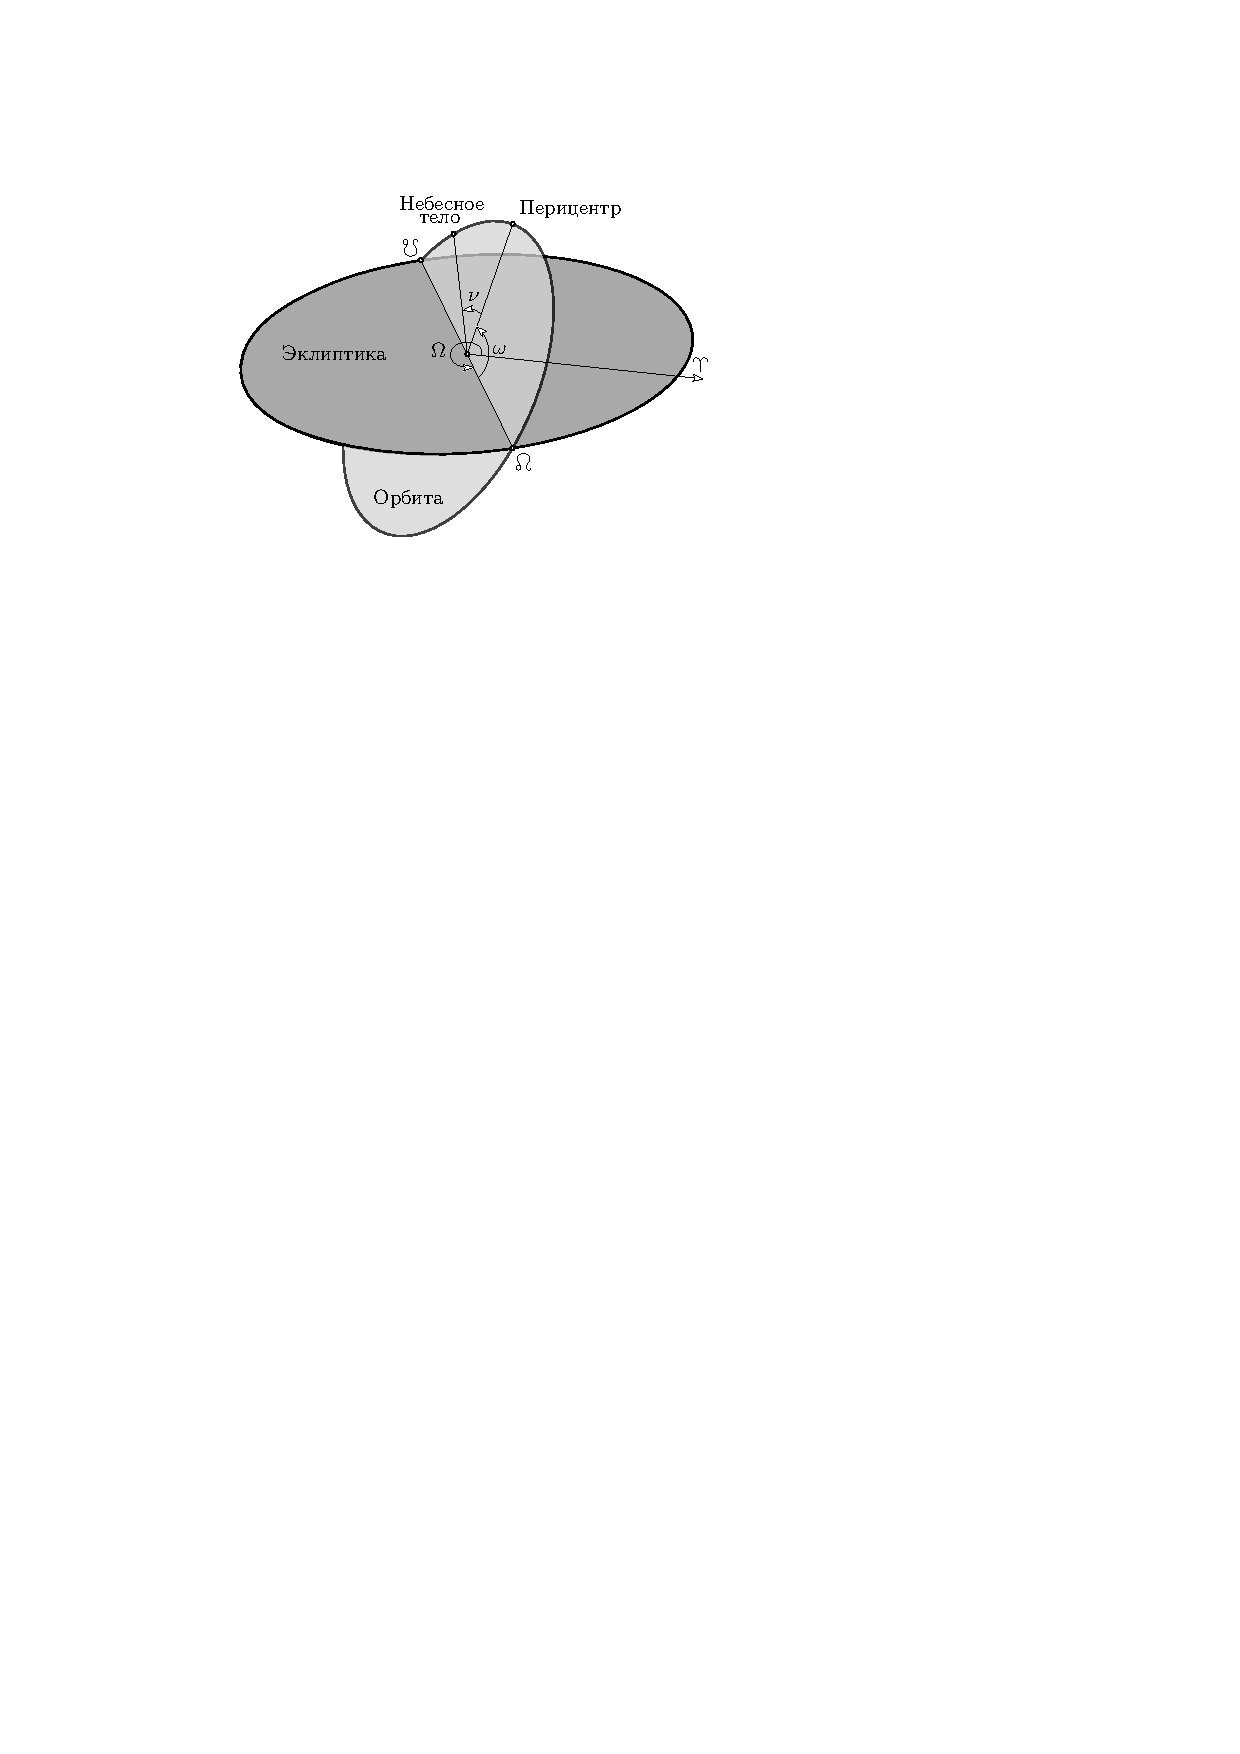
\includegraphics[width=.45\tw]{orbit-elem}
	\captionof{figure}{Кеплеровы элементы орбиты}
	\label{fig:orb-elem}
\end{wrapfigure}
небесного тела в пространстве в задаче двух тел: \imp{большая полуось} ($a$), \imp{эксцентриситет} ($e$), \imp{наклонение} ($i$), \imp{аргумент перицентра} ($\omega$), \imp{долгота восходящего узла} ($\Omega$), \imp{средняя аномалия} ($M$). Первые два определяют форму орбиты, третий, четвёртый и пятый~--- ориентацию плоскости орбиты по отношению к базовой системе координат, связанной с эклиптикой, последний~--- положение тела на орбите~(см.~Рис.\,\ref{fig:orb-elem}).

\term{Наклонение}~--- это угол между плоскостью орбиты небесного тела и плоскостью эклиптики.

\term{Аргумент перицентра}~--- угол между направлениями на восходящий узел орбиты и на перицентр при наблюдении из притягивающего центра.

\term{Долгота восходящего узла}~--- угол в плоскости эклиптики между направлением на точку весеннего равноденствия и восходящий узел орбиты. Отсчитывается против часовой стрелки от направления на точку весеннего равноденствия.

\term{Средняя аномалия} для тела, движущегося по невозмущённой орбите~--- произведение его среднего движения и интервала времени после прохождения перицентра.

\term{Узлы орбиты}~--- точки пересечения орбиты и плоскости эклиптики. \imp{Восходящий узел}~--- точка, в которой тело пересекает плоскость эклиптики при движении в северноим направлении, а \imp{нисходящий}~--- в южном.

\term{Истинная аномалия}~($\nu$)~--- угол между радиус-вектором и направлением на перицентр.
